

\section{Классификация состояний марковской цепи на основе свойств неразложимости и апериодичности}

\textbf{Автор:} Мамыко Ксения Юрьевна, Б-01-001

\begin{definition}\label{oduvan_def_1} (марковская цепь в широком смысле)  Пусть $(\Omega, \mathscr{F}, {(\mathscr{F}_n)}_{n \geq 0}, \mathbf{P})~-$ фильтрованное вероятностное пространство и $(E, \mathscr{E})~-$ фазовое пространство. Последовательность $X = {(X_n)}_{n \geq 0}$ случайных элементов $X_n = X_n(\omega)$, заданных на $(\Omega, \mathscr{F}, {(\mathscr{F}_n)}_{n \geq 0}, \mathbf{P})$, принимающих значения в $E$ и являющихся
$\mathscr{F}_n/\mathscr{E}$ -измеримыми, $n \geq 0$, называется последовательностью величин, связанных \emph{марковской зависимостью (марковской цепью, цепью Маркова) в широком смысле}, если для любых $n \geq 0$ и $B \in \mathscr{E}$ выполнено \emph{марковское свойство в широком смысле}:

\begin{equation}\label{oduvan_eq_1}
    \mathbf{P}(X_{n+1} \in B| \mathscr{F}_n)(\omega) = \mathbf{P}(X_{n+1} \in B| X_n(\omega))
\end{equation}

\end{definition}

Если ${\mathscr{F}_n}^X = \sigma (X_0, X_1, \ldots, X_n)$ есть $\sigma$-алгебра, порожденная величинами $X_0, X_1, \ldots, X_n$, то, поскольку ${\mathscr{F}_n}^X \subseteq \mathscr{F}_n$, а $X_n~- {\mathscr{F}_n}^X$-измеримы, из (\ref{oduvan_eq_1}) получаем \emph{марковское свойство в узком смысле} (или просто \emph{марковское свойство}):

\begin{equation}\label{oduvan_eq_2}
    \mathbf{P}(X_{n+1} \in B| {\mathscr{F}_n}^X)(\omega) = \mathbf{P}(X_{n+1} \in B| X_n(\omega)) 
\end{equation}

Для наглядности это свойство записывают часто в
таком виде:

\begin{equation}\label{oduvan_eq_3}
    \mathbf{P}(X_{n+1} \in B|X_0(\omega), \ldots, X_n(\omega)) = \mathbf{P}(X_{n+1} \in B| X_n(\omega)) 
\end{equation}

Выведенное из (\ref{oduvan_eq_1}) марковское свойство в узком смысле (\ref{oduvan_eq_2}) подсказывает целесообразность введения понятия марковской зависимости и в том
случае, когда a priori не выделяется поток ${(\mathscr{F}_n)}_{n \geq 0}$.

\begin{definition}\label{oduvan_def_2}(марковская цепь) Пусть $((\Omega, \mathscr{F}, \mathbf{P}))$ вероятностное пространство, $(E, \mathscr{E})$ фазовое пространство. Последовательность $X = {(X_n)}_{n \geq 0}$ случайных элементов $X_n = X_n(\omega)$, принимающих значения
в $E$ и являющихся $\mathscr{F}/\mathscr{E}$-измеримыми, называется последовательностью величин, связанных \emph{марковской зависимостью (марковской цепью, цепью Маркова)}, если для любых $n \geq 0$ и $B \in \mathscr{E}$ выполнено \emph{марковское свойство в узком смысле} (\ref{oduvan_eq_2}).
\end{definition}

\begin{remark} Введение с самого начала фильтрованного вероятностного пространства, на котором определялась марковская цепь \emph{в широком смысле}, оказывается полезным во многих вопросах, где поведение
систем рассматривается в зависимости от того или иного «потока информации» ${(\mathscr{F}_n)}_{n \geq 0}$. Например, может случиться, что у «двумерного» процесса $(X, Y) = (X_n, Y_n)_{n \geq 0}$ первая компонента $X = {(X_n)}_{n \geq 0}$, не будучи марковской в смысле определения (2), тем не менее является марковской в смысле определения (\ref{oduvan_def_1}) с ${\mathscr{F}_n} = {\mathscr{F}_n}^{X, Y}, n \geq 0$. В элементарном же изложении теории марковских цепей поток ${(\mathscr{F}_n)}_{n \geq 0}$ обычно не вводится и за
основу принимается определение \ref{oduvan_def_2}.
\end{remark}

Будем предполагать, что рассматриваемая марковская цепь имеет
\emph{счетное} множество состояний $E = \{1, 2, \ldots\}$ и переходные вероятности $p_{ij}, i,j \in E$. Матрицу (таблицу), образованную этими переходными вероятностями, будем обозначать $\mathbb {P} = \Vert p_{ij} \Vert$ или, в более развернутой форме,

\[ \mathbb {P} = \begin{Vmatrix}
  p_{11}& p_{12}& p_{13}& \cdots\\
  p_{21}& p_{22}& p_{23}& \cdots\\
  \cdots & \cdots & \cdots& \cdots\\
  p_{i1}& p_{i2}& p_{i3}& \cdots\\
  \cdots & \cdots & \cdots& \cdots
\end{Vmatrix}. \]

(Вместо $\Vert \cdot \Vert$ для матриц часто бывает удобнее писать ($\cdot$).)

Приводимая далее классификация состояний марковских цепей полностью определяется \emph{алгебраическими} свойствами матриц переходных вероятностей $\mathbb{P}$ и их степеней $\mathbb{P}^{(n)}$, $n \geq 1$.

Матрица переходных вероятностей $\mathbb{P}$ полностью определяет \emph{одношаговые} переходы из состояния в состояние. Матрицы же $\mathbb{P}^{(n)} = \Vert {p_{ij}}^{(n)} \Vert$ определяют (в силу марковского свойства) переходы за \emph{n шагов}.

Скажем, матрица

\[ \mathbb{P} = \begin{pmatrix}
  1/2& 1/2\\
  0& 1
\end{pmatrix}\]

и соответствующий ей граф показывают, что определяемое
ими \emph{движение} «частицы», блуждающей по состояниям 0 и 1, таково, что
за один шаг возможен переход 0 $\rightarrow$ 1 (с вероятностью 1/2), но переход 1 $\rightarrow$ 0 невозможен. Ясно, что переход 1 $\rightarrow$ 0 невозможен и за любое число шагов, что видно, конечно, и из структуры матриц

\[ \mathbb{P}^{(n)} = \begin{pmatrix}
  2^{-n} & 1 - 2^{-n}\\
  0& 1
\end{pmatrix}, \]

показывающей, что ${p_{10}}^{(n)} = 0$ при любом $n \geq 1$.

В этом примере состояние 1 является таким, что в него можно \emph{войти} (из состояния 0), но нельзя из него \emph{выйти}.

Рассмотрим граф на рис.~\ref{fig::oduvan_pic_1}, по которому легко восстановить и соответствующую матрицу переходов $\mathbb{P}$. Из вида этого графа ясно, что здесь
имеется три состояния (левая часть рисунка), выйдя из которых, обратно
вернуться невозможно.

С точки зрения «будущего» поведения «частицы», блуждающей в соответствии с данным графом, эти три состояния \emph{несущественны} (и называются \emph{несущественными}) по той указанной причине, что из них \emph{возможен
выход}, но в них \emph{невозможно возвращение}.

\begin{figure}[h!]
			\centering
			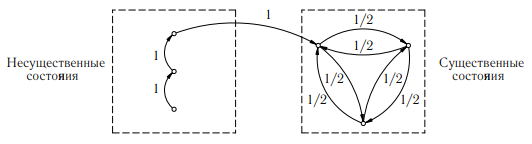
\includegraphics[width=0.6\linewidth]{oduvanchik_i_pic_1.png}
			\caption{~}
			\label{fig::oduvan_pic_1}
\end{figure}

Такие «несущественные» состояния, не представляющие интереса,
можно сразу отбросить, сосредоточив все внимание на классификации
лишь оставшихся «\emph{существенных}» состояний.

Чтобы расклассифицировать существенные состояния или группы
таких состояний, нам понадобится ряд определений.

\begin{definition} Говорят, что состояние $j$ \emph{достижимо} из состояния $i$ (обозначение: $i \rightarrow j$), если найдется такое $n \geq 0$, что ${p_{ij}}^{(n)} > 0$ (${p_{ij}}^{(0)} = 1$, если $i = j$, и 0, если $i \neq j$).

Состояния $i$ и $j$ называются \emph{сообщающимися} (обозначение: $i \leftrightarrow j$), если $i \rightarrow j$ и $j \rightarrow i$, т. е. они являются \emph{взаимно достижимыми}.
\end{definition}

\begin{lemma} Свойство сообщаемости «$\leftrightarrow$» (взаимной достижимости) есть отношение эквивалентности состояний (марковской цепи
с матрицей переходных вероятностей $\mathbb{P}$).
\end{lemma}

\begin{proof}По определению отношения эквивалентности (в данном случае отношения «$\leftrightarrow$») надо проверить его рефлексивность
($i\leftrightarrow i$), симметричность (если $i \leftrightarrow j$, то $j \leftrightarrow i$) и транзитивность (если
$i \leftrightarrow j$, $j \leftrightarrow k$, то $i \leftrightarrow k$).

Первые два свойства следуют непосредственно из определения сообщаемости состояний. Транзитивность вытекает из уравнения Колмогорова - Чепмена: если ${p_{ij}}^{(n)} > 0$, ${p_{jk}}^{(m)} > 0$, то

\[{p_{ik}}^{(n+m)} = \sum_{l \in E} {p_{il}}^{(n)} {p_{lk}}^{(m)} \geq {p_{ij}}^{(n)} {p_{jk}}^{(m)} > 0,\]

т. е. $i \rightarrow k$. Аналогично, $k \rightarrow i$. Тем самым, $i \leftrightarrow k$. \end{proof}

Будем относить все сообщающиеся между собой состояния $i, j, k, \ldots$
($i \leftrightarrow j$, $j \leftrightarrow k$, $k \leftrightarrow i$, $\ldots$) к одному \emph{классу}. Тогда любые такие классы состояний или совпадают, или же не пересекаются. Следовательно, отношение \emph{сообщаемости} разбивает все множество (существенных) состояний $E$ на конечное или счетное число непересекающихся множеств $E_1, E_2, \ldots (E = E_1 + E_2 + \ldots)$.

Эти множества будем называть \emph{неразложимыми классами} (существенных сообщающихся) состояний. Марковскую цепь, все состояния которой образуют \emph{один} неразложимый класс, будем называть \emph{неразложимой}.

Для иллюстрации введенных понятий рассмотрим цепь с пространством
состояний $E = \{ 1, 2, 3, 4, 5\}$ и матрицей переходных вероятностей

\[
\newcommand*{\temp}{\multicolumn{1}{r|}{}}
\mathbb{P} = \begin{pmatrix}
  1/3 & 2/3 &\temp & 0 & 0 & 0\\
  1/3 & 2/3 &\temp &0 & 0 & 0\\ \cline{1-6}
  0 & 0 &\temp &0 & 1 & 0\\
  0 & 0 &\temp &1/2 & 0 & 1/2\\
  0 & 0 &\temp &0 & 1 & 0
\end{pmatrix}
=
\begin{pmatrix}
  \mathbb{P}_1&\temp &0\\ \hline
  0&\temp &\mathbb{P}_2
\end{pmatrix}
.
\]

Граф этой цепи с \emph{пятью} состояниями имеет следующий вид:

\begin{figure}[h!]
    \centering
    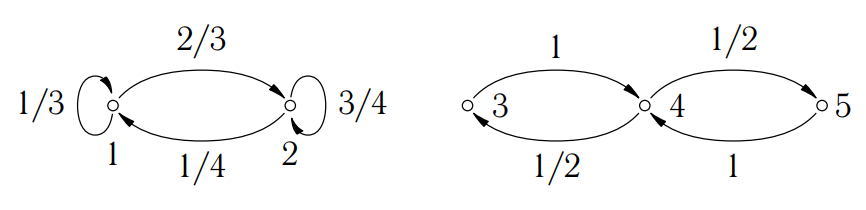
\includegraphics[width=0.5\linewidth]{oduvanchik_i_pic_2.png}
    \caption{~}
    \label{fig::oduvan_pic_2}
\end{figure}

\begin{wrapfigure}{r}{0.4\textwidth}
                \centering
			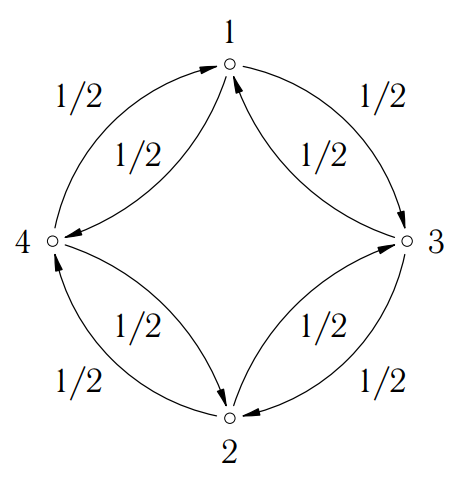
\includegraphics[width=0.6\linewidth]{oduvanchik_i_pic_3.png}
			\caption{Пример марковской цепи с периодом d = 2}
			\label{fig::oduvan_markov_chain_exm}
\end{wrapfigure}

Ясно, что у рассматриваемой цепи есть \emph{два} неразложимых класса $E_1 = \{1, 2\}$, $E_2 = \{3, 4, 5\}$, и исследование ее свойств сводится к исследованию свойств каждой из двух цепей, множествами состояний которых
являются множества $E_1$ и $E_2$, а матрицы переходных вероятностей равны соответственно $\mathbb{P}_1$ и $\mathbb{P}_2$.

Рассмотрим теперь какой-нибудь неразложимый класс $E$. Для примера пусть им будет класс, изображенный на рис.~\ref{fig::oduvan_pic_2}.



Заметим, что здесь возвращение в каждое состояние возможно лишь за \emph{четное} число шагов, переход в соседнее состояние$~-$ за \emph{нечетное} число шагов, а матрица переходных вероятностей имеет блочную структуру:

\[
\newcommand*{\temp}{\multicolumn{1}{r|}{}}
\mathbb{P} = 
\begin{pmatrix}
  0 & 0 & \temp &1/2 & 1/2\\
  0 & 0 & \temp &1/2 & 1/2\\ \cline{1-5}
  1/2 & 1/2& \temp & 0 & 0\\
  1/2 & 1/2&\temp & 0 & 0
\end{pmatrix}
.\]

Отсюда видно, что класс $E = \{1, 2, 3, 4\}$ разбивается на два подкласса
$C_0 =\{1, 2\}$ и $C_1 =\{3, 4\}$, обладающих следующим свойством \emph{цикличности}:
за один шаг из $C_0$ «частица» непременно переходит в $C_1$, а из $C_1$$~-$ в $C_0$.

Приведенный пример показывает, что, по-видимому, и в общем случае можно дать соответствующую классификацию \emph{неразложимых} классов состояний на \emph{циклические подклассы}.

С этой целью нам понадобятся некоторые определения и один факт из
теории чисел.

\begin{definition} Пусть $\varphi = (\varphi_1, \varphi_2, \ldots)~-$ некоторая последовательность неотрицательных чисел $\varphi_n \geq 0, n \geq 1$. \emph{Периодом} последовательности $\varphi$ (обозначение: $d(\varphi)$) называется число 

\[d(\varphi) = \text{НОД} \{n \geq 1 : \varphi_n > 0\},\]

где НОД$(M_{\varphi})$ есть \emph{Наибольший Общий Делитель} множества $M_{\varphi}$ тех индексов $n \geq 1$, для которых $\varphi_n > 0$; если $\varphi_n = 0, n \geq 1$, то 
$M_{\varphi} = \oslash$ и НОД($M_{\varphi}$) полагается равным нулю.
\end{definition}

По-другому можно сказать, что последовательность $\varphi$ имеет период
$d(\varphi)$, если из того, что $\varphi_n > 0$, следует, что $d(\varphi)$ делит $n$ (т. е. $n$ должно иметь вид $d(\varphi)k$ с некоторым $k \geq 1$) и $d(\varphi)$ является наибольшим среди всех тех чисел $d$, которые обладают таким свойством (т. е. таких, что $n=dl$ с некоторым целым $l \geq 1$).

Так, например, последовательность $\varphi = (\varphi_1, \varphi_2, \ldots)$ такая, что $\varphi_{4k} > 0$ для $k = 1, 2, \ldots$ и $\varphi_n = 0$ для $n \neq 4k$, имеет период $d(\varphi) =$ 4, а не 2, хотя $\varphi_{2l} > 0$ для $l = 2, 4, 8$.

\begin{definition} Говорят, что последовательность $\varphi = (\varphi_1, \varphi_2, \ldots)$ \emph{апериодическая}, если ее период $d(\varphi) = 1$.
\end{definition}

Следующий элементарный результат из теории чисел будет в дальнейшем полезен при классификации состояний по свойству цикличности.

\begin{lemma} Пусть $M~-$ некоторое множество неотрицательных
целых чисел ($M \subseteq E$), замкнутое относительно сложения и такое,
что НОД$(M) = 1$. Тогда при некотором $n_0$ все числа $n \geq n_0$ будут принадлежать $M$.
\end{lemma}

Применим эту лемму к множеству $M = M_{\varphi}$, беря в качестве последовательности $\varphi = (\varphi_1, \varphi_2, \ldots)$ последовательность $({p_{jj}}^{(1)}, {p_{jj}}^{(2)}, \ldots)$ или последовательность $({p_{jj}}^{(d)}, {p_{jj}}^{(2d)}, \ldots)$, $d \geq 1$, где $j~-$ некоторое состояние марковской цепи, имеющей матрицу переходных вероятностей $\mathbb{P} = \Vert p_{ij} \Vert$, а ${p_{jj}}^{(n)}~-$ элемент матрицы ${\mathbb{P}}^{(n)}, n \geq 1, {\mathbb{P}}^{(1)} = \mathbb{P}$. (При этом будем говорить, что
состояние $j$ имеет период $d(j)$, если $d(j)$ есть период последовательности
$({p_{jj}}^{(1)}, {p_{jj}}^{(2)}, \ldots)$.)  Тогда получим следующий результат.

\begin{theorem} \emph{Пусть состояние $j$ имеет период $d = d(j)$.}

\emph{Если $d = 1$, то найдется такое $n_0 = n_0 (j)$, что для всех $n \geq n_0$ переходные вероятности ${p_{jj}}^{(n)} > 0$.}

\emph{Если $d > 1$, то найдется такое $n_0 = n_0 (j, d)$, что для всех $n \geq n_0$ переходные вероятности ${p_{jj}}^{(nd)} > 0$.}

\emph{Если $d \geq 1$ и ${p_{ij}}^{(m)} > 0$ для некоторых $i \in E$ и $m \geq 1$, то найдется такое $n_0 = n_0(j, d, m)$, что ${p_{ij}}^{(m + nd)} > 0$  для всех $n \geq n_0$.}
\end{theorem}

Приведем теперь теорему, показывающую, что \emph{период} состояний неразложимого класса обладает свойством «однотипности».

\begin{theorem} \emph{Пусть ${E}_* =\{i, j, \ldots \}~-$ некоторый неразложимый класс (сообщающихся) состояний из множества $E$.}
\emph{Все состояния такого класса являются «однотипными» в том
смысле, что они имеют один и тот же период (обозначаемый $d(E_*)$
и называемый периодом класса $E_*$).}
\end{theorem}

\begin{proof}
Пусть $i, j \in E_*$. Тогда найдутся такие $k$ и $l$, что ${p_{ij}}^{(k)} > 0$ и ${p_{ji}}^{(l)} > 0$. Но тогда в силу уравнения Колмогорова$~–$ Чепмена
\[{p_{ii}}^{(k + l)} = \sum_{a \in E} {p_{ia}}^{(k)} {p_{ai}}^{(l)} \geq {p_{ij}}^{(k)} {p_{ji}}^{(l)} > 0,\]
и, значит, $k + l$ должно делиться на $d(i)~-$ период состояния $i \in E_*$.

Пусть $d(j)~-$ период состояния $j \in E_*$ и $n$ таково, что ${p_{jj}}^{(n)} > 0$. Тогда $n$ должно делиться на $d(j)$ и так как
\[{p_{ii}}^{(n + k + l)} \geq {p_{ij}}^{(k)} {p_{jj}}^{(n)} {p_{ji}}^{(l)} > 0,\]
то $n + k + l$ делится на $d(i)$. Но $k + l$ делится на $d(i)$, а значит, $n$ делится на $d(i)$ и поскольку $d(j) = \text{НОД}\{ n: {p_{jj}}^{(n)} > 0\}$, то $d(i) \leq d(j)$.

По симметрии $d(j) \leq d(i)$, и, следовательно, $d(i) = d(j)$.
\end{proof}

Если множество состояний $E_* \subseteq E$ образует неразложимый класс
(сообщающихся состояний) и $d(E_*) = 1$, то о таком классе говорят как об
\emph{апериодическом классе} состояний.

Рассмотрим теперь случай $d(E_*) \geq 1$.

Переходы из состояния в состояние внутри такого класса могут осуществляться весьма причудливым образом (как в рассмотренном выше примере марковской цепи с периодом $d(E_*) =2$; см. рис. \ref{fig::oduvan_pic_2}).

\begin{wrapfigure}{r}{0.4\textwidth}
                \centering
			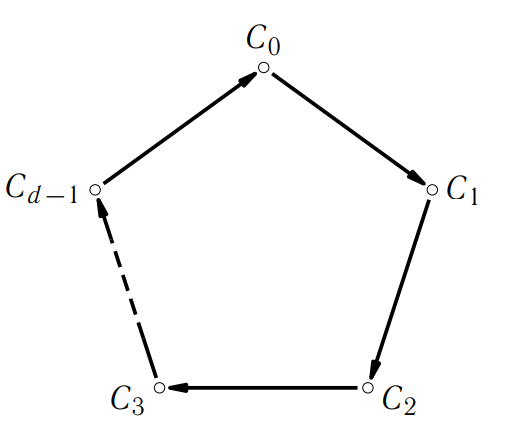
\includegraphics[width=0.6\linewidth]{oduvanchik_i_pic_4.png}
			\caption{Движение по циклическим подклассам}
			\label{fig::oduvan_cycle_motion}
\end{wrapfigure}
Оказывается, однако, что в этих переходах, из одной группы состояний в другую, имеет место вполне определенная «\emph{цикличность}»:


\begin{theorem} \emph{Пусть $E_*$ –– неразложимый класс состояний, $E_* \subseteq E$, с периодом $d = d(E_*) > 1$. Тогда найдутся $d$ групп состояний $C_0, C_1, \ldots , C_{d-1}$, называемых циклическими подклассами $(E_* = C_0 + C_1 + \ldots + C_{d-1})$, характеризуемые тем, что в моменты времени $n = p + kd$ с $p = 0, 1, \ldots , d - 1$ и
$k=0, 1, \ldots$ «частица» будет находиться в подклассе $C_p$ с переходом
в следующий момент в $C_{p+1}$, затем в $C_{p+2}, \ldots$, в $C_{d - 1}$, из $C_{d-1}$ в $C_0$ и т. д.}
\end{theorem}


\begin{proof}
    Зафиксируем некоторое состояние $i_0 \in E_*$ и введем следующие подклассы:
    \[
    C_0 = \{j \in E_* : \text{если}~ {p_{i_0j}}^{(n)} > 0, \text{то}~ n = kd,~ k = 0, 1, \ldots\}
    \]
    \[
    C_1 = \{j \in E_* : если~ {p_{i_0j}}^{(n)} > 0, \text{то}~ n = kd + 1,~ k = 0, 1, \ldots\}
    \]
    \[
    \ldots\]
    \[
    C_{d-1} = \{j \in E_* : \text{если}~ {p_{i_0j}}^{(n)} > 0,~ \text{то}~ n = kd + (d-1), k = 0, 1, \ldots\}
    \]

    Ясно, что $E_* =C_0 + C_1 + \ldots + C_{d-1}$. Покажем, что движение «частицы» из подкласса в подкласс осуществляется описанным в теореме способом; см. рис. \ref{fig::oduvan_markov_chain_exm}.
    
В самом деле, рассмотрим некоторое состояние $i \in C_p$, и пусть состояние $j \in E_*$ таково, что $p_{ij} > 0$. Покажем, что тогда непременно $j \in C_{(p+1) (\text{mod}~ d)}.$

Пусть $n$ таково, что ${p_{i_0j}}^{(n)} > 0$. Тогда $n$ может быть представлено в виде $n = p + kd$ с некоторыми $p = 0, 1, \ldots, d - 1$ и $k = 0, 1, \ldots$ Значит, $n \equiv p$ (mod $d$), и поэтому $n + 1 \equiv (p + 1) \cdot$ $\cdot$(mod $d$). Отсюда следует, что ${p_{i_0j}}^{(n+1)} > 0$ (по определению периода $d = d(E_*)$), и, значит, $j \in C_{(p+1) (\text{mod}~ d)}$, что и
требовалось установить.
\end{proof}

Заметим, что из приведенных рассуждений следует, что матрица $\mathbb{P}$ переходных вероятностей имеет \emph{блочную} структуру:

\begin{figure}[h!]
    \centering
    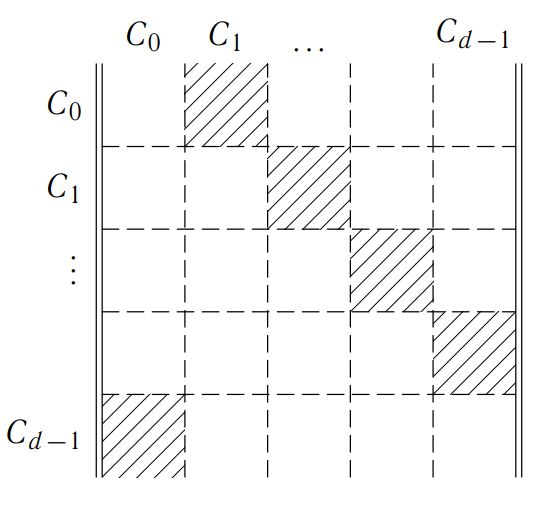
\includegraphics[width=0.3\linewidth]{oduvanchik_i_pic_5.png}
\end{figure}

Предположим сейчас, что блуждающая «частица», эволюция которой
управляется матрицей $\mathbb{P}$, начинает свое движение из некоторого состояния
в подклассе $C_0$. Тогда в каждый из моментов времени $n = p +kd$ эта «частица» будет находиться (в силу определения подклассов $C_0, C_1, \ldots, C_{d-1}$)
в множестве $C_p$.

Следовательно, с каждым таким множеством состояний $C_p$ можно связать \emph{новую} марковскую цепь с матрицей переходов $\Vert {p_{ij}}^{(d)} \Vert$, где $i, j \in C_p$. Эта новая цепь будет \emph{неразложимой} и \emph{апериодической}.

\begin{figure}[h!]
			\centering
			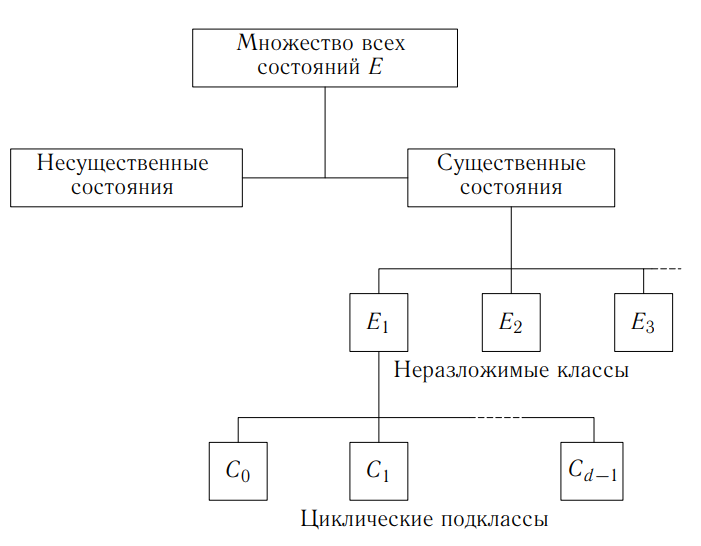
\includegraphics[width=0.6\linewidth]{oduvanchik_i_pic_6.png}
			\caption{Классификация состояний марковской цепи по арифметическим свойствам
вероятностей ${p_{ij}}^{(n)}$}
			\label{ris lab}
\end{figure}

Таким образом, принимая во внимание проведенную классификацию
(на несущественные и существенные состояния, неразложимые классы и
циклические подклассы; см. сводный рис. \ref{fig::oduvan_cycle_motion}), можно сделать такой вывод:

\begin{center}
  При исследовании вопросов предельного поведения переходных вероятностей\\
  ${p_{ij}}^{(n)},~ n \geq 1,~ i,j \in E$, определяющих блуждание «марковской частицы»,\\ можно ограничиваться рассмотрением лишь того случая, когда фазовое\\ пространство $E$ само является \emph{единственным неразложимым апериодическим\\ классом} состояний.
\end{center}

В этом предположении саму марковскую цепь $X = (X_n)_{n \geq 0}$ с таким
фазовым пространством и матрицей переходных вероятностей $\mathbb{P}$ называют
\emph{неразложимой и апериодической}.

